\section{UI}

The project includes two Tkinter-based interfaces that mirror the same dark,
card-based visual language.

The first interface is the input browser. It lets the user inspect the exact
image and prompt passed into the benchmark pipeline, along with the loading
steps used to construct the sample. This is useful for checking that each
dataset row is rendered and prepared as intended before inference begins.

The second interface is the results browser. It loads the saved JSON reports
produced by the benchmark runs and presents them with run-level summaries,
filters, and per-sample inspection. The goal is to make the outputs easy to
scan without losing the underlying prediction, reference, and telemetry data.

\begin{figure}[H]
    \centering
    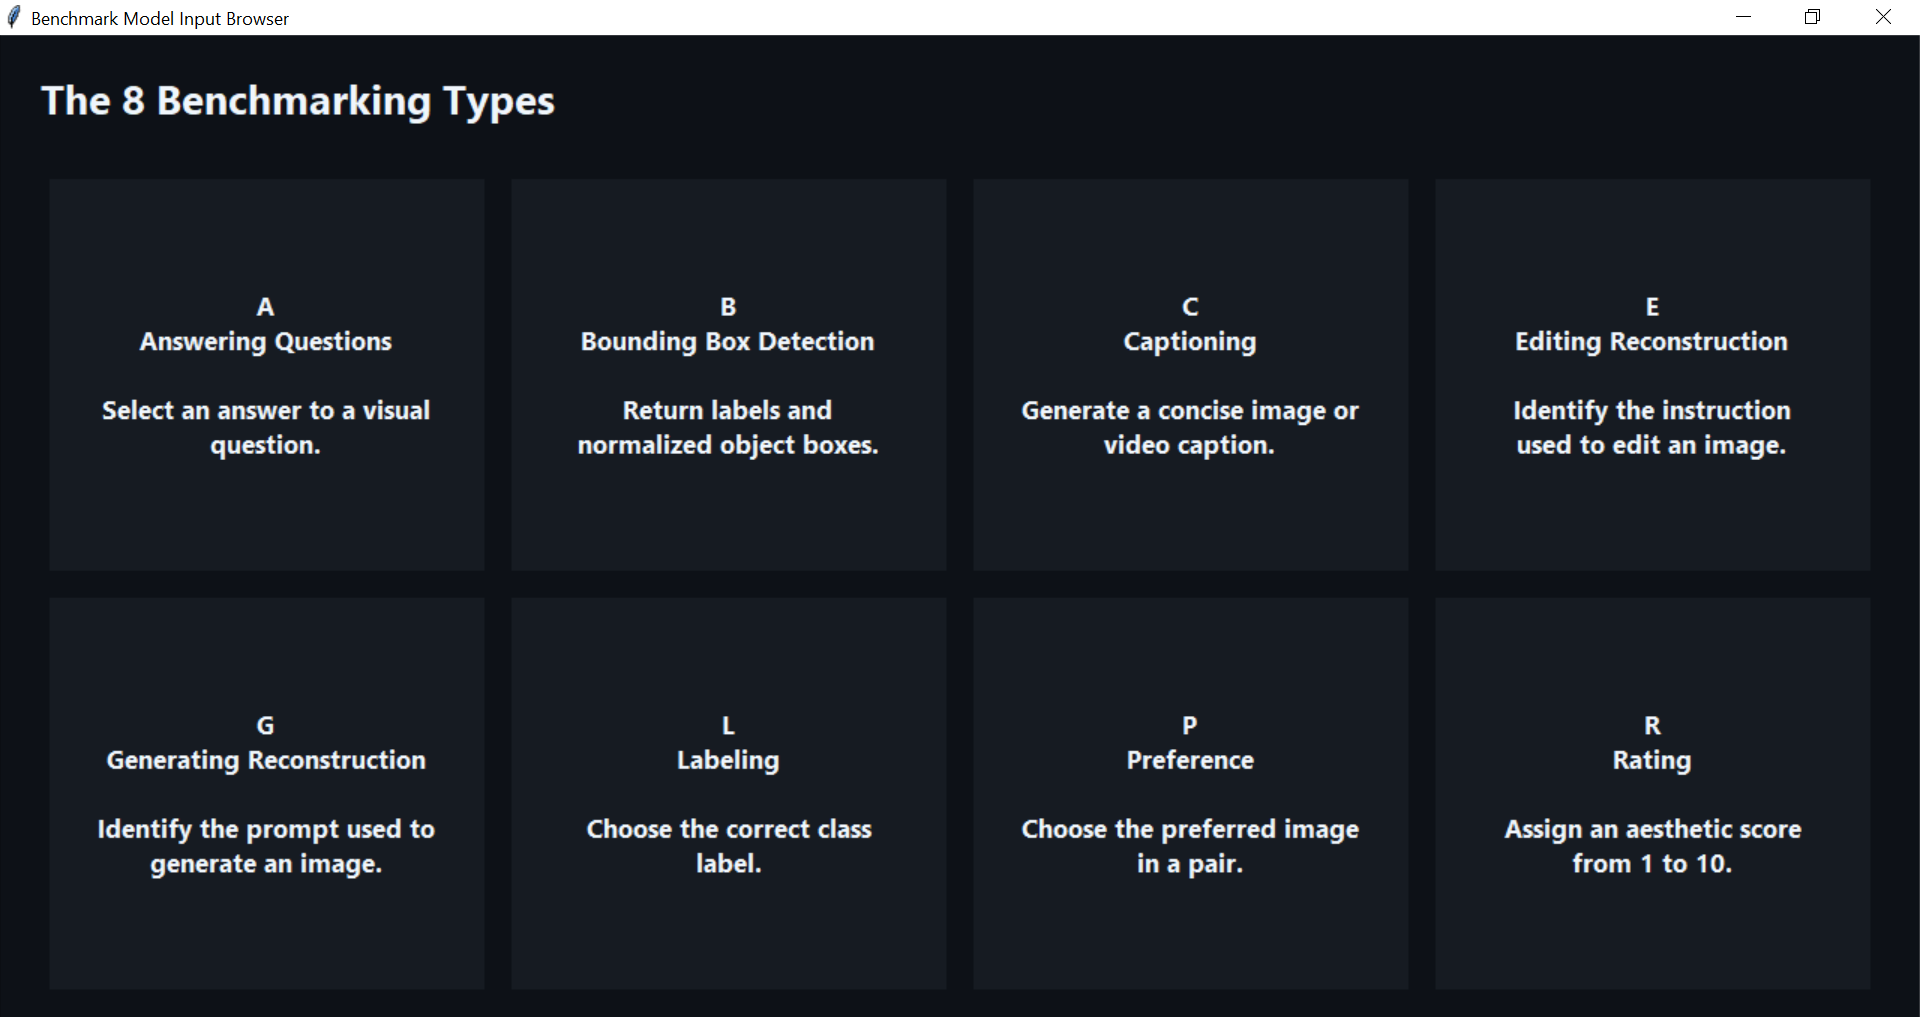
\includegraphics[width=0.92\textwidth]{../ui/ui.PNG}
    \caption{Input browser used to inspect the exact benchmark image and prompt before model inference.}
    \label{fig:ui-input}
\end{figure}

\begin{figure}[H]
    \centering
    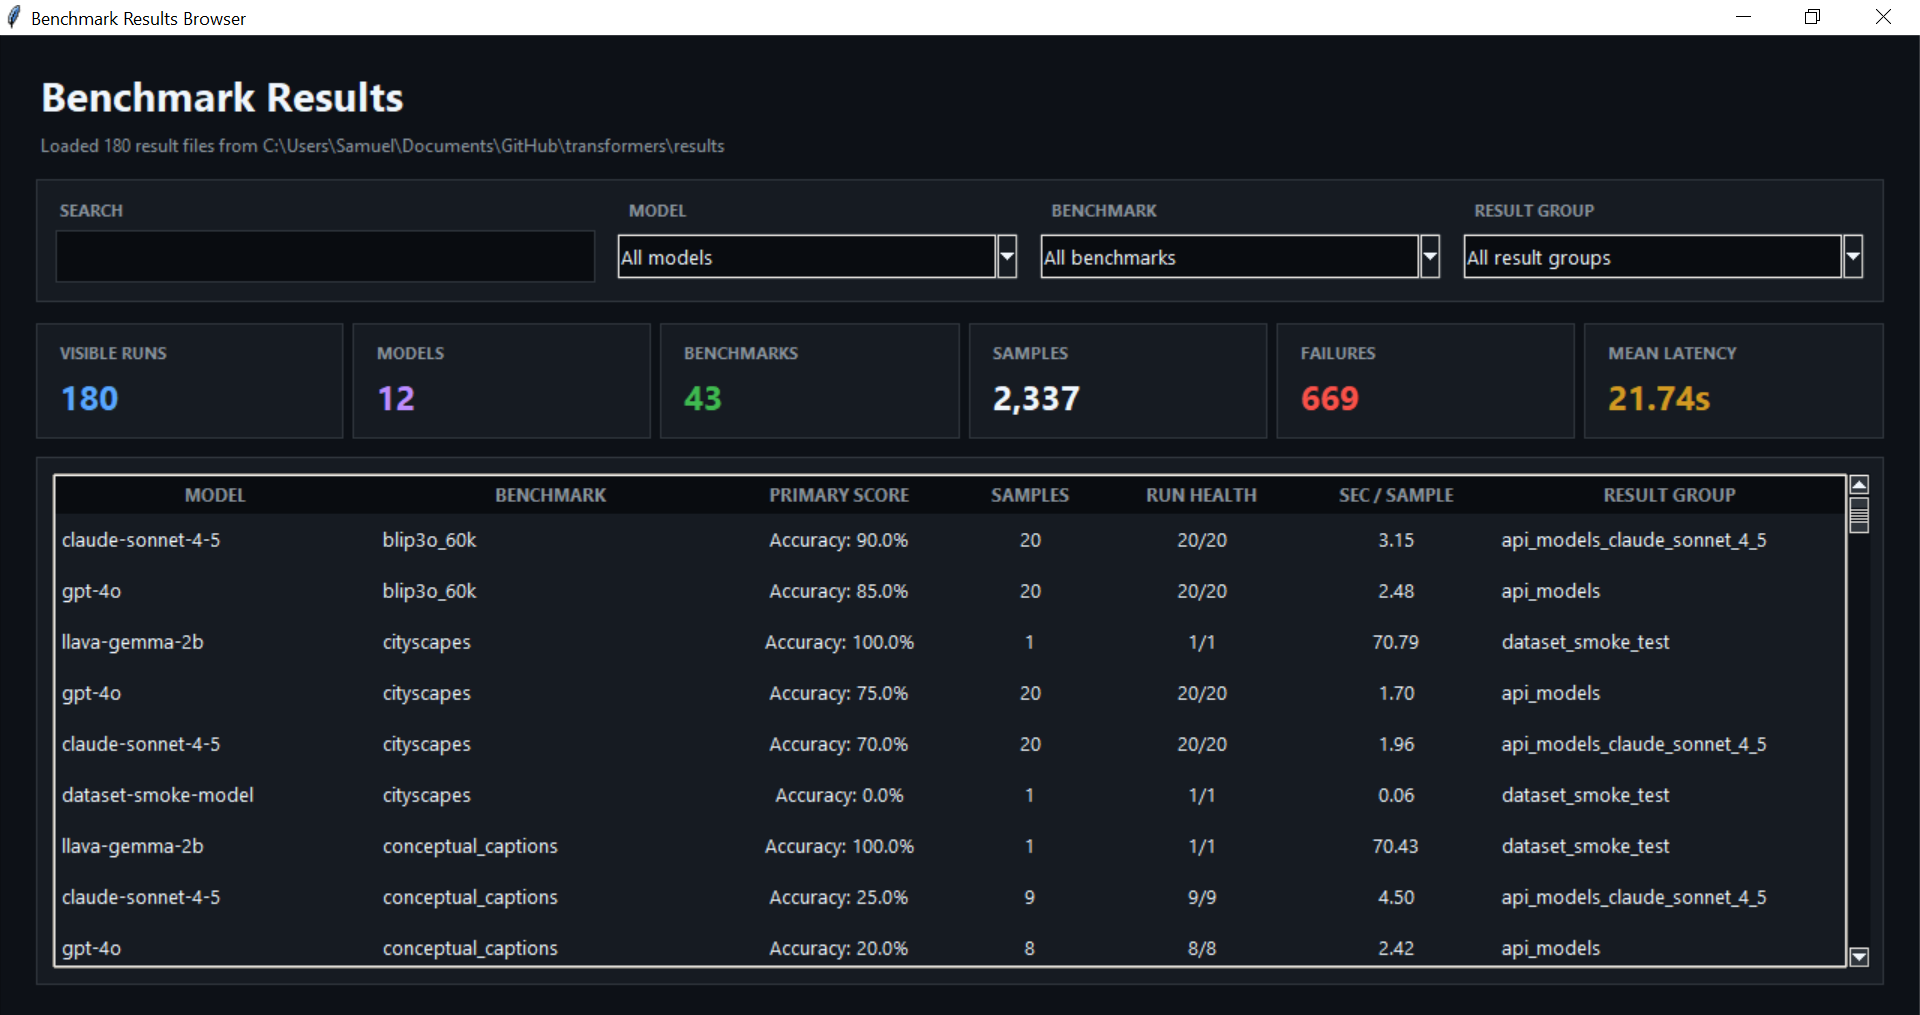
\includegraphics[width=0.92\textwidth]{../ui/ui_results.PNG}
    \caption{Results browser used to inspect benchmark outputs, run summaries, and per-sample details.}
    \label{fig:ui-results}
\end{figure}
